\documentclass[11pt]{article}

\usepackage{amsmath,mathtools,siunitx,amssymb}
\usepackage[a4paper,left=1.5cm,right=1.5cm,top=2cm,bottom=2cm]{geometry}
\usepackage{float,subcaption,graphicx}
\usepackage{enumitem,pifont}
\renewcommand{\labelitemi}{\ding{228}}
\renewcommand{\labelitemii}{\ding{229}}
\renewcommand{\labelitemiii}{\ding{225}}
\setlist[itemize]{noitemsep}
\usepackage[dvipsnames]{xcolor}
\usepackage{color,hyperref}
\hypersetup{colorlinks=true}

\graphicspath{{images/}}

\begin{document}
{\Large\bfseries Project Notes}
\section{Replicating results}
\begin{itemize}
    \item Here are my plots for replicating what we did in first term:
        \begin{figure}[H]
            \centering
            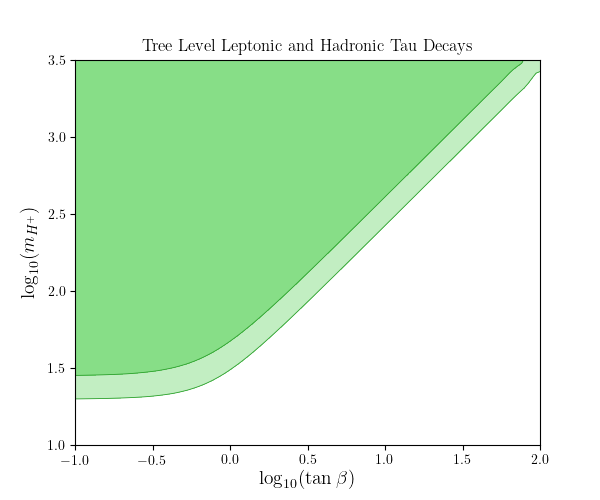
\includegraphics[width=0.45\textwidth]{leps_plot.png}
            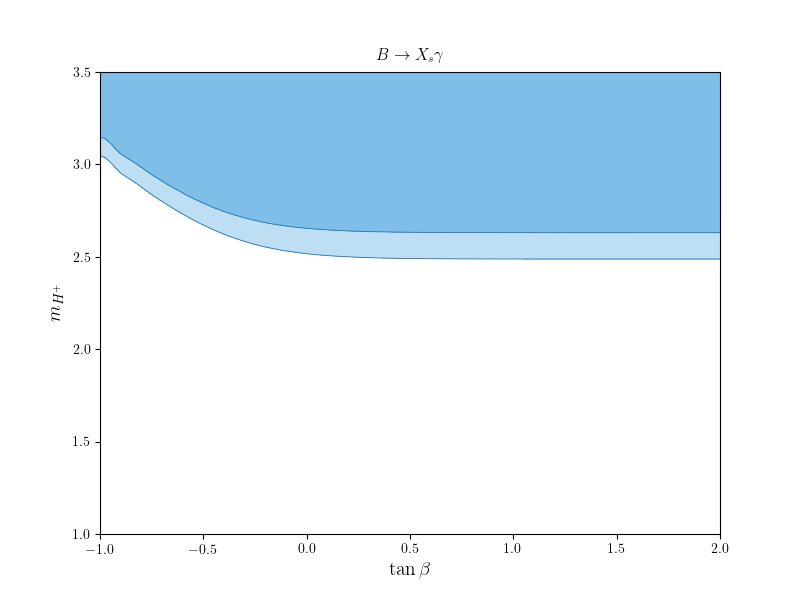
\includegraphics[width=0.45\textwidth]{bsgamma_plot.png}
            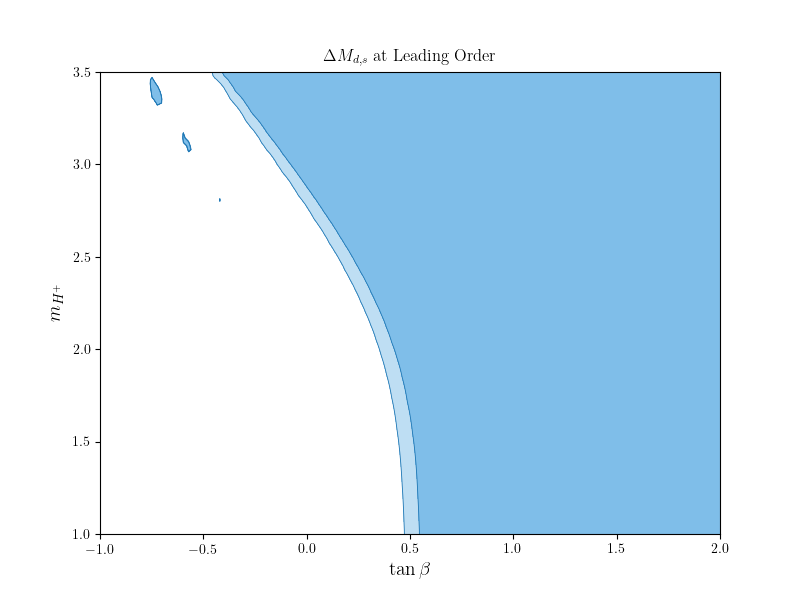
\includegraphics[width=0.45\textwidth]{bmix_plot.png}
            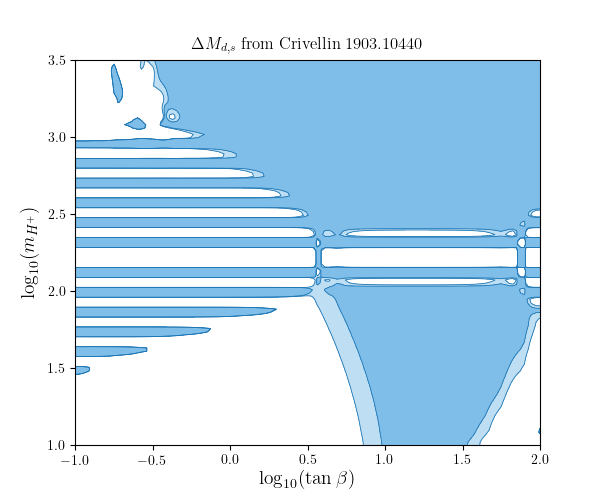
\includegraphics[width=0.45\textwidth]{bcriv_plot.png}
            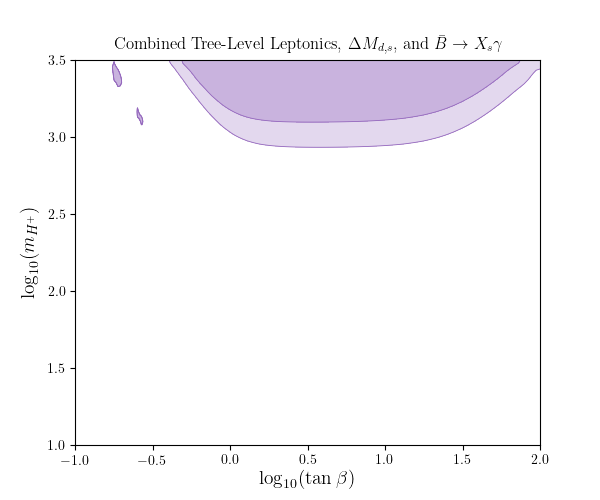
\includegraphics[width=0.45\textwidth]{comb1_plot.png}
        \end{figure}
    \item Like Oliver, the main difference seems to be with $b\to s\gamma$ where it fits higher than before -- \textbf{the combined fit yields $m_{H^+}\gtrsim970\,$GeV at $2\sigma$ compared to $m_{H^+}\gtrsim\,$GeV in my previous fits}
    \item \textit{Note: all the plots here are showing contours for $1,2\sigma$}
    \item I have modified the SM value in flavio for $b\to s\gamma$ to fit the current result of $(3.40\pm0.17)e^{-4}$ but still got this higher result
    \item It seems like it could be down to how flavio fits, but we would need to confirm this if we want to leave it as is
    \item I have also included the fit for B mixing from higher-order expressions in \href{https://arxiv.org/pdf/1903.10440}{Crivellin 1903.10440} to show the difference -- the gap we find around $m_{H^+}\sim m_t(m_t)$ is due to divergences in the loop functions for this value
    \item Adding in $B_{s,d}\to\mu\mu$ and $\mathcal{R}(D^{(*)})$ yields similar results to what I had before
        \begin{figure}[H]
            \centering
            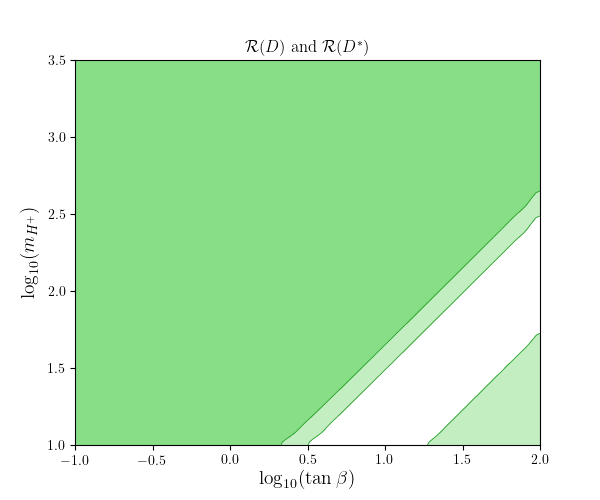
\includegraphics[width=0.45\textwidth]{rd_both.png}
        \end{figure}
    \item $\mathcal{R}(D)$ and $\mathcal{R}(D^*)$ are fitting simultaneously it seems right now, which wasn't what we had before, so looking at individual plots:
        \begin{figure}[H]
            \centering
            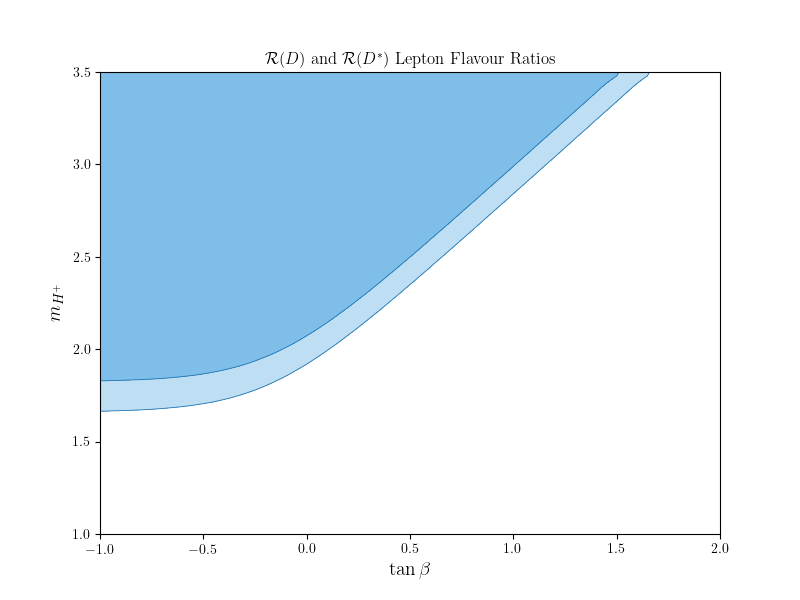
\includegraphics[width=0.45\textwidth]{rd_plot.png}
            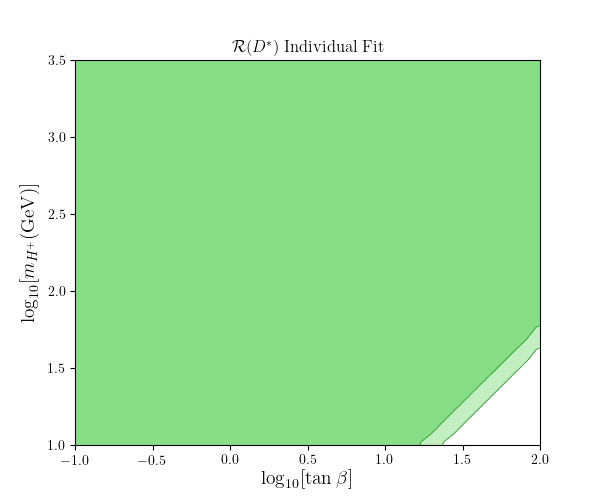
\includegraphics[width=0.45\textwidth]{rdst_plot.png}
        \end{figure}
    \item It appears that both of them do fit individually which is not what we had before -- I'm not quite sure why this is the case currently
    \item For $B_{s,d}\to\mu\mu$, the left diagram is approximating $m_{H^+}\sim m_{H^0}$ which is the rough limit James has from the obliques, and the right diagram is fixing $m_{H^0}=1500\,$GeV
    \item Using the convention from 1903.10440 for the trilinear couplings means that instead of using $M=m_{12}/(\sin\beta\cos\beta)$ as I did previously, you use $\lambda_3$ from the 2HDM potential
    \item The two trilinear couplings we have to consider are
        \begin{align*}
            \lambda_{h^0 H^+ H^-} &= v\sin(\beta-\alpha)\lambda_3, &
            \lambda_{H^0 H^+ H^-} &= v\cos(\beta-\alpha)\lambda_3 
        \end{align*}
    \item In the alignment limit which I have been using so far for these, $\sin(\beta-\alpha)=1$, so we only have to consider $\lambda_{h^0 H^+ H^-}$ 
        \begin{figure}[H]
            \centering
            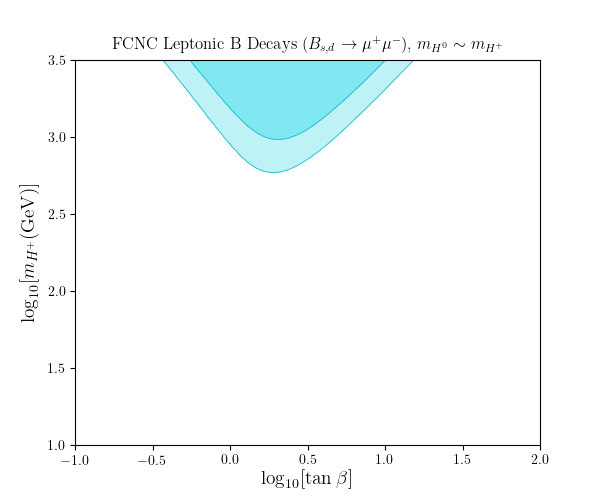
\includegraphics[width=0.45\textwidth]{bmumu_apx.png}
            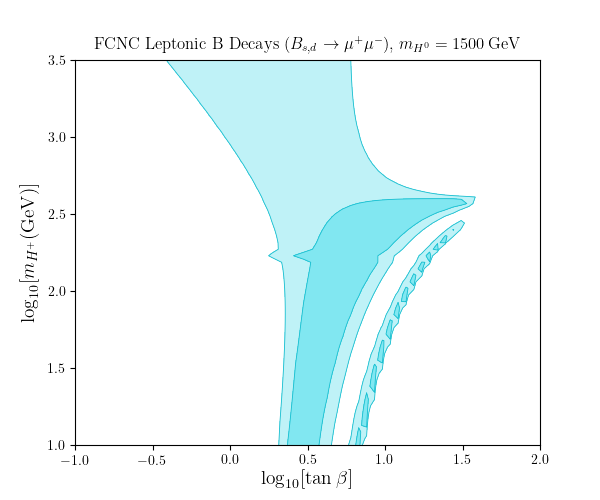
\includegraphics[width=0.45\textwidth]{bmumu_fix.png}
        \end{figure}
    \item The contributions from the trilinear coupling seems to be minimal anyway, varying $\lambda_3$ from $0.01\to2$ doesn't change the results to any noticeable level, so for now I have set $\lambda_3=0.1$, but it's probably better to fit it properly at some point
    \item The coupling only contributes to $C_S$ and $C_P$ operators so far which only impact $B\to\mu\mu$
    \item Checking the combined fit for all these observables to compare to my overall project work (bar the inclusion of James' obliques):
        \begin{figure}[H]
            \centering
            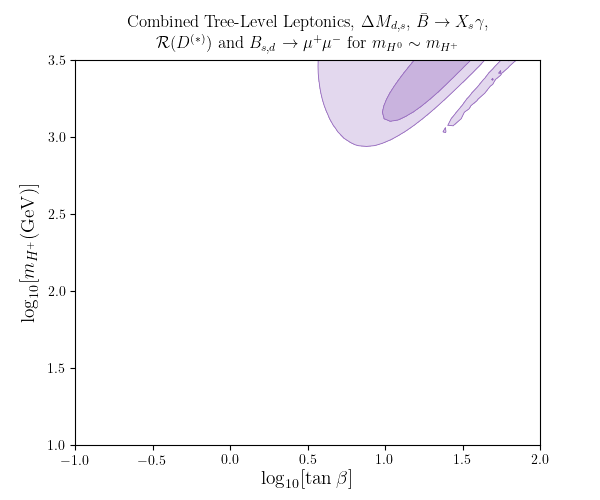
\includegraphics[width=0.45\textwidth]{comb2_apx.png}
            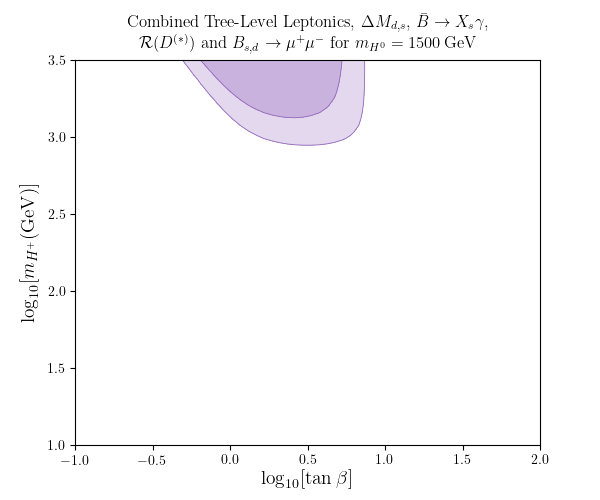
\includegraphics[width=0.45\textwidth]{comb2_fix.png}
        \end{figure}
    \item Left is approximating $m_{H^+}\sim m_{H^0}$ as above for $B\to\mu\mu$ (can't compare to project directly as didn't use this limit); right is fixing $m_{H^0}=1500\,$GeV
    \item For the right, we have $m_{H^+}\gtrsim970\,$GeV and $\tan\beta\lesssim7$; in my project for this, I had $m_{H^+}\gtrsim500\,$GeV and $\tan\beta\lesssim21$
\end{itemize}

\section{New Observables and To Do}
\begin{itemize}
    \item Also started looking at the tree-level semileptonic decays 
    \item For semileptonics and leptonics, I think the WC contributions work out the same, e.g. for $b\to u\mu\nu_\mu$ (using the subscript convention from \href{https://wcxf.github.io/assets/pdf/WET.flavio.pdf}{flavio's WET basis})
        \begin{align*}
            \mathcal{O}_{SR} = -\frac{4G_F}{\sqrt{2}}V_{ub}(\bar{u}_Lb_R)(\bar{\mu}_R\nu_{\mu L}) &\to C_{SR} = \frac{m_u}{m_{H^+}^2} \\
            \mathcal{O}_{SL} = -\frac{4G_F}{\sqrt{2}}V_{ub}(\bar{u}_Rb_L)(\bar{\mu}_L\nu_{\mu R}) &\to C_{SL} = \frac{m_b\tan^2\beta}{m_{H^+}^2} 
        \end{align*}
    \item For the tree-level leptonics, this transforms to $r_H$ from \href{https://arxiv.org/pdf/0907.5135.pdf}{0907.5135}, and looks to give the right results for semileptonics (including being used for the $\mathcal{R}(D)$s above) 
    \item So providing the SM calculations for the semileptonics are fine, it's quite simple to fit these too:
        \begin{figure}[H]
            \centering
            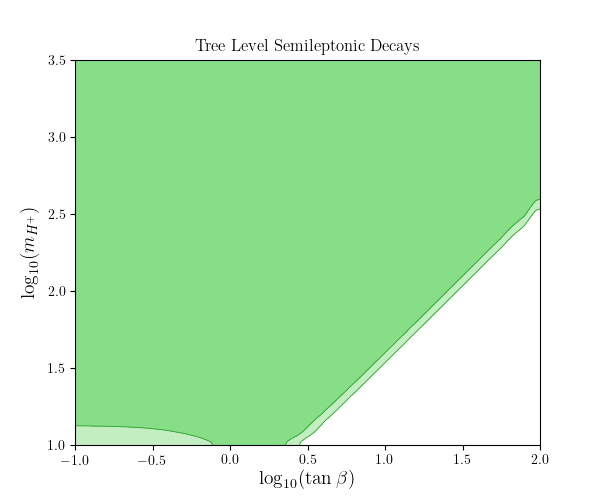
\includegraphics[width=0.45\textwidth]{sls_plot.png}
        \end{figure}
    \item The next thing is to look at $R_K$ and $R_{K^{*0}}$ 
    \item From \href{https://arxiv.org/pdf/1704.05340.pdf}{1704.05340}, the operators needed for the $R_K$s are $C_7,C_7',C_9,C_9',C_{10},C_{10}'$ for both $bs\mu\mu$ and $bsee$
    \item All these can be got from \href{https://arxiv.org/pdf/1903.10440.pdf}{1903.10440} -- already have the formulae for $C_{10}^{(')}$s from $B\to\mu\mu$ calculations
    \item For both $m_{H^+}\sim m_{H^0}$ and $m_{H^0}=1500\,$GeV as I looked at $B\to\mu\mu$, we get no constraint in our parameter space from $R_K$ and $R_{K^{*0}}$ (although I still need to check through all the formulae again for mistakes):
        \begin{figure}[H]
            \centering
            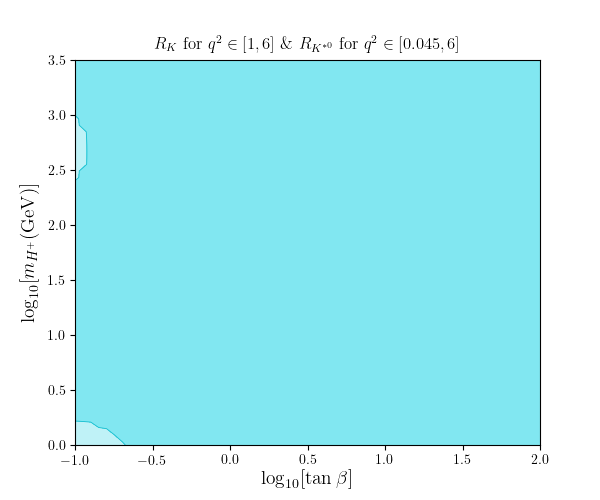
\includegraphics[width=0.45\textwidth]{rks_plot.png}
        \end{figure}
    \item I want to check in literature as well for the $R_K$s in 2HDM Type II to see if there's any fits that include these to see what results have been found historically to give some at least a rough idea of what should be expected
    \item I will also look at fitting $b\to s\gamma$ using the expressions for $C_7,C_8$ in 1903.10440 since $C_7$ is in $R_K$s anyway
    \item I need to do the fits including $B\to\mu\mu$ in the wrong sign limit too and compare to my previous results
\end{itemize}


\end{document}
